\documentclass[a4paper,12pt]{report}
\usepackage[utf8]{inputenc}
\usepackage[francais]{babel}
\usepackage{fancyhdr}
\usepackage{graphicx}
\usepackage{tikz}
\usetikzlibrary{calc}
\usepackage{listings}
\usepackage{xcolor}
\definecolor{grey}{rgb}{0.9,0.9,0.9}
\usepackage{titlesec}
\usepackage{verbatim}
\usepackage{listings}
\usepackage{textcomp}
\usepackage{hyperref}
\usepackage{longtable}
\usepackage{colortbl}
\usepackage{amssymb}

\frenchbsetup{StandardLists=true}
\newcommand{\marge}{18mm}
\usepackage[left=\marge,right=\marge,top=\marge,bottom=\marge]{geometry}
\pagestyle{fancy}
\setlength{\headheight}{14pt}
\chead{
   Badache Yassine
  \hspace{13em}
  \vspace{0.9em}
  Sujet 70: Serveur de jeux au tour par tour}
\renewcommand{\headrulewidth}{1pt}
\linespread{1}
\setlength{\columnseprule}{0.2pt}
\definecolor{javakeyword}{rgb}{0,0,0.5}
\definecolor{javastring}{rgb}{0,0.5,0}
\definecolor{javacomment}{rgb}{0.5,0.5,0.5}
\lstdefinestyle{java}{
   language=Java, basicstyle=\footnotesize,       % the size of the fonts that are used for the code
  numbers=left,                   % where to put the line-numbers
  numberstyle=\tiny\color{gray},  % the style that is used for the line-numbers
  stepnumber=1,                   % the step between two line-numbers. If it's 1, each line
                                  % will be numbered
  numbersep=5pt,                  % how far the line-numbers are from the code
  backgroundcolor=\color{white},  % choose the background color. You must add \usepackage{color}
  showspaces=false,               % show spaces adding particular underscores
  showstringspaces=false,         % underline spaces within strings
  showtabs=false,                 % show tabs within strings adding particular underscores
  frame=single,                   % adds a frame around the code
  rulecolor=\color{black},        % if not set, the frame-color may be changed on line-breaks within not-black text (e.g. commens (green here))
  tabsize=2,                      % sets default tabsize to 2 spaces
  captionpos=b,                   % sets the caption-position to bottom
  breaklines=true,                % sets automatic line breaking
  breakatwhitespace=false,        % sets if automatic breaks should only happen at whitespace
  title=\lstname,                 % show the filename of files included with \lstinputlisting;
   stringstyle=\color{javastring},
   keywordstyle=\color{javakeyword}\ttfamily\textbf,
   commentstyle=\color{javacomment}\ttfamily\textit
 }
 
 \bibliographystyle{plain}
 \frenchbsetup{StandardLists=true}
 
 %%%%%%%%%%%%%%%%%%%%%%%%%%%%%%%%%%%%%%% PDF INFO 
 %%%%%%%%%%%%%%%%%%%%%%%%%%%%%%%%%%%%%%%%%%%%%%%%
 \hypersetup{
 	pdfauthor   = {Yassine Badache},
 	pdftitle    = {Rapport de PJI (Projet individuel)},
 	pdfsubject  = {Serveur de jeux au tour par tour},
 	pdfkeywords = {Lille Serveur Jeux Yassine Badache PJI},
 	pdfcreator  = {PDFLaTeX},
 	pdfproducer = {PDFLaTeX}
 }
 %%%%%%%%%%%%%%%%%%%%%%%%%%%%%%%%%%%%%%%%%%%%%%%%
 
\author{Yassine Badache}
\title{}
\titleformat{\chapter}[hang]{\bf\huge}{\thechapter}{2pc}{}
\begin{document}
	
	\makeatletter
\begin{titlepage}
\centering
{\LARGE \textbf{\textsc{Projet Individuel}}}\\
\vspace{20em}
{\LARGE \textsc{Sujet 70: Serveur de jeux au tour par tour
}}\\


\vspace{6em}
{\LARGE Etudiant: Yassine Badache\\
	\vspace{2em}
		Encadrants: Yoann DUFRESNE, Gauvin MARQUET}\\


\vspace{15em}

\begin{tikzpicture}[remember picture,overlay]

\node [below left,xshift=-1cm, yshift=4cm] at (current page.south east){
\includegraphics[scale=0.6]{images/ustl1.jpg}};

\end{tikzpicture}
\end{titlepage}
\makeatother

\sloppy
	\input{thanks.tex}

	\tableofcontents	
	\newpage
	\setcounter{page}{1}
% Début de document

	\chapter{Introduction}

	L'an dernier, deux étudiants en Master 1 Informatique ont développé un \textit{framework} permettant de développer, à l'aide d'automates, des jeux au tour par tour. Les jeux ainsi implémentés peuvent héberger une partie de manière indépendante, contenant les protocoles de communication entre elle-même et le client.
	\\
	
	Le but principal de ce PJI était de concevoir un composant logiciel permettant d'accéder aux différents jeux implémentés, et de les instancier par ce biais. Ceci permettrait alors un accès simplifié aux jeux développés et une centralisation des ressources nécessaires à son bon fonctionnement.
	\\
	
	Au-delà de l'accès public aux ressources, c'est notamment dans une vision plus 'interne' qu'a été proposé ce projet individuel. En effet, l'aboutissement final de ce composant logiciel serait d'héberger des intelligences artificelles, s'affrontant sur les supports développés via le \textit{framework} de l'an dernier.
	\\
	\chapter{Conception}

Le programme développé ici est supposé répondre à un besoin bien précis, c'est-à-dire l'accessibilité d'une ressource bien définie et son utilisation, que ce soit par un utilisateur humain ou par une intelligence artificielle développée spécifiquement pour le jeu souhaité. La première partie de ce projet a donc été dédiée à la conception de ce projet par les besoins d'un utilisateur quel qu'il soit.\\

\section{Diagrammes de séquence}

Ci-dessous sont détaillés les scénarios d'usage du logiciel, ainsi que leurs diagrammes de séquence associés. C'est l'ensemble de ces éléments qui nous a permis par la suite de cerner le cœur de ce qui est attendu à la fin de ce sujet.\\

Nous nommerons ici "entité" l'utilisateur: en effet, en plus d'un utilisateur humain, administrateur ou non, une intelligence artificielle devrait également être en mesure d'accéder à notre service afin d'instancier une partie ou rejoindre une partie existante, se confrontant alors à une autre intelligence artificielle ou à un joueur déjà présent en jeu.

\newpage
\subsection{Premier cas d'utilisation: créer une partie d'un jeu}	
	
	\begin{figure}[!ht]
		\center
		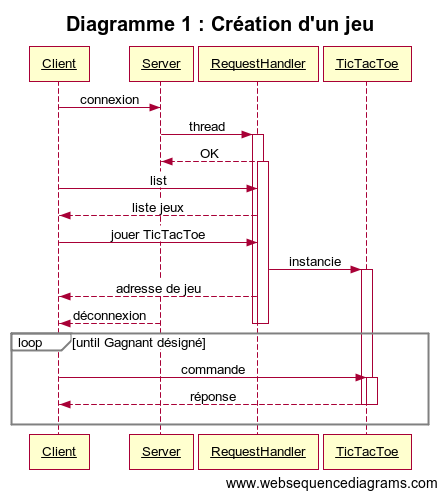
\includegraphics[scale=0.7]{images/sequence/diagramme_scenario1.png}
		\caption{Le premier cas d'utilisation, basique}
	\end{figure}
	
	\underline{Description}\\
	
	\textit{Une entité souhaite jouer à un jeu. Elle lance donc le client, qui lui permet de se connecter 
		au serveur. Elle entre la commande “list” qui lui permet de voir quels jeux sont disponibles. 
		Parmi eux, elle choisit le TicTacToe, qui est alors instancié du fait qu'aucune partie n'est active. Le serveur lui renvoie l'adresse de jeu, à laquelle l'entité se pourra se connecter que si suffisamment de joueurs souhaitent participer.}\\
	
	\vspace{3em}
	Ce cas d'utilisation pose les bases de l'utilisation de notre serveur: on l'utilise principalement pour jouer, et on attend que suffisamment de joueurs soient en attente pour ce jeu afin d'en instancier une.
	\newpage
	
	\subsection{Deuxième cas d'utilisation: rejoindre une partie existante}
	\begin{figure}[!ht]
		\center
		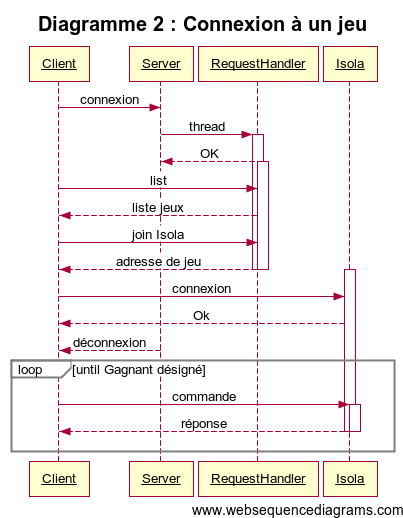
\includegraphics[scale=0.7]{images/sequence/diagramme_rejoindre.png}
		\caption{Rejoindre une partie}
	\end{figure}
	
	\underline{Description}\\
	
	\textit{Une entité souhaite jouer à un jeu. Elle lance donc le client, qui lui permet de se connecter 
		au serveur. Elle entre la commande “list” qui lui permet de voir quels jeux sont disponibles. 
		Parmi eux, elle choisit de jouer à l'Isola. Des parties étant déjà en cours, le serveur lui renvoie l'adresse d'une des parties, à laquelle l'entité se connecte pour ensuite jouer à l'Isola.}\\
	
	\vspace{3em}
	Ce cas d'utilisation introduit la notion non plus de création d'une instance de jeu, mais bien de connexion à une partie existante. Il faut donc définir des moyens de contrôler et de retenir les jeux étant actuellement instanciés pour pouvoir effectuer la connexion entre le client et le jeu en question.
	\newpage
	
	\subsection{Troisième cas d'utilisation: ajouter un jeu sur le serveur}
	\begin{figure}[!ht]
		\center
		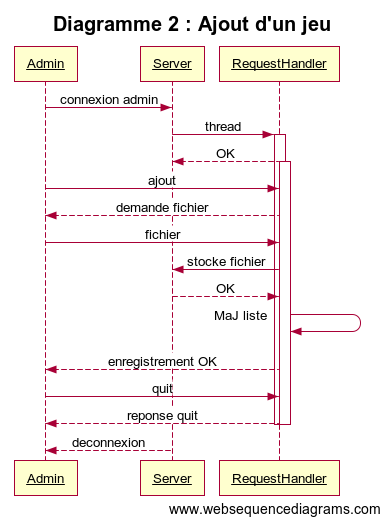
\includegraphics[scale=0.7]{images/sequence/diagramme_ajout.png}
		\caption{Ajout d'un jeu}
	\end{figure}
	
	\underline{Description}\\
	
	\textit{Un administrateur se connecte au service en ligne, via un pseudonyme et mot de passe associés. Il ajoute ensuite un jeu via la commande associée, et le fichier du jeu lui est demandé: il le choisir, et valide son choix. Il choisit un nom pour le jeu choisi, et le serveur stocke ledit fichier dans ses données, mettant  à jour la liste des jeux disponibles. Une fois l'enregistrement effectué, l'administrateur entre la commande 'quit' et se voit déconnecté du serveur.}\\
	
	\vspace{3em}
	
	Ce troisième cas d'utilisation introduit un autre acteur possible, soit l'administrateur. Entrent en compte des problèmes de sécurité liés au statut privilégié, l'enregistrement de fichiers et la saisie de celui-ci.
	\newpage
	
	\subsection{Quatrième cas d'utilisation: quitter une partie en cours}
	\begin{figure}[!ht]
		\center
		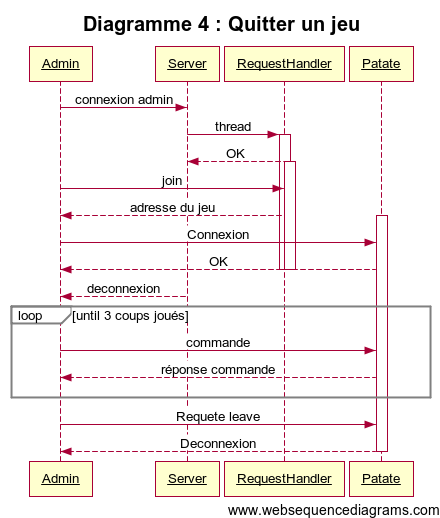
\includegraphics[scale=0.7]{images/sequence/diagramme_leave_cas1.png}
		\caption{Quitter une partie}
	\end{figure}
	
	\underline{Description}\\
	
	\textit{Une entité souhaite participer à une partie. Elle entre donc la commande 'join Patate', qui lui permettra de se connecter à une partie actuellement en cours de la Patate chaude. L'adresse du jeu lui est renvoyée et elle s'y connecte. Cependant, au bout de trois coups joués, elle se rend compte qu'elle ne souhaite pas continuer à jouer. Elle entre donc la commande 'leave', et se voit immédiatement déconnectée du jeu en cours.}\\
	
	\vspace{3em}
	
	Lorsque l'on joue à un jeu, il est aussi bénéfique de savoir comment le quitter, pour des raisons diverses. Cependant, ce cas d'utilisation ne concerne pas vraiment le serveur développé par nos soins: en effet, une fois connecté au jeu, l'interaction avec le \textit{software} devient nulle, et la commande permettant de quitter une partie devrait alors être partie intégrante du système de jeu.
	\newpage


	
\section{Automate à états finis en découlant}

De ces diagrammes de séquence découlent quelques questions primaires qui ont dû être traités en tout premier lieu, avant encore d'entamer la conception de notre programme, à commencer par sa représentation 'graphique'. Le schéma suivant montre le modèle final de notre programme ainsi que tous ses états et transitions possibles.\\


\begin{figure}[!ht]
	\center
	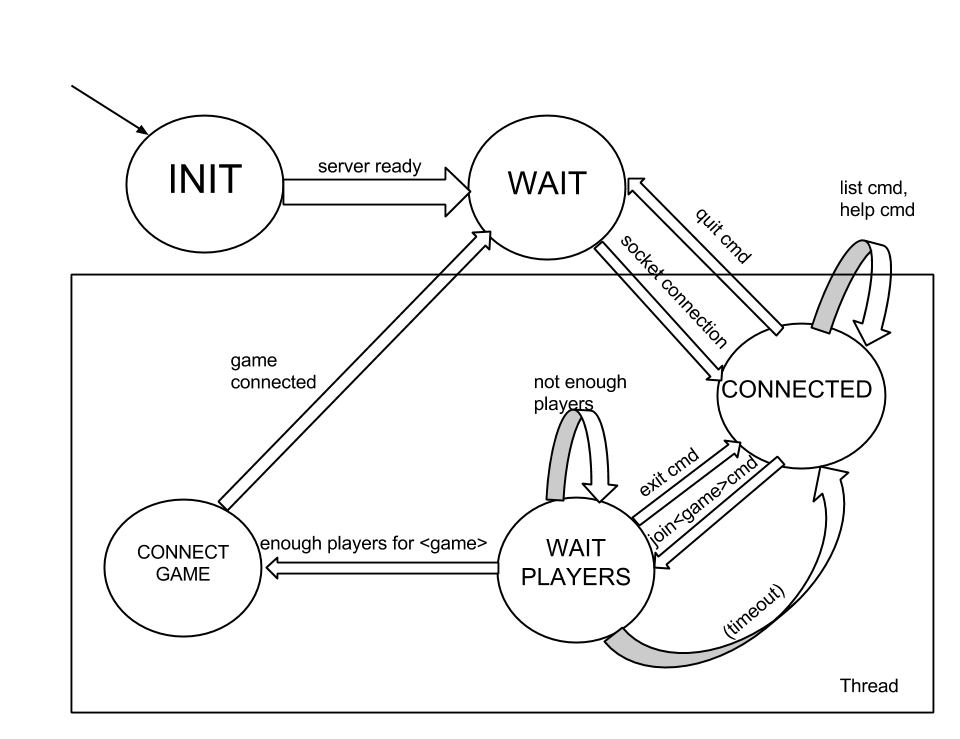
\includegraphics[scale=0.5]{images/state_machine_server.png}
	\caption{L'automate décrivant notre serveur}
\end{figure}


\underline{Explication}\\


\begin{itemize}
	\item \textbf{INIT}\\
	La phase d'initialisation du serveur, qui devrait être plus ou moins instantanée.
	\vspace{1em}
	
	
	\item \textbf{WAIT}\\
	Une fois l'initialisation terminée et le serveur prêt, celui-ci entre dans une phase d'attente, où il attendra la connexion d'un client. Dans le cadre de ce projet, le client est une simple application développée en parallèle, mais à l'avenir, le logiciel est prévu pour soutenir n'importe quel type de client.
	\newpage
	
	
	\item \textbf{CONNECTED}\\
	Le client, une fois connecté, est en mesure d'envoyer des commandes et en recevoir les réponses. Le format utilisé est le JSON, pour la compréhension sur multiples supports et son universalité.
	Si l'utilisateur entre les commandes 'list' ou 'help', il reste dans l'état courant, CONNECTED. Il ne changera d'état qu'à deux conditions:
	
	\begin{itemize}
		\item La commande 'quit', pour se déconnecter du service
		\item La commande 'join (game)' afin de d'accéder au service principal du serveur, soit la connexion à un jeu.
	\end{itemize}
	\vspace{1em}
	
	
	\item \textbf{WAIT PLAYERS}\\
	Cet état est un état intermédiaire entre l'envoi de la commande et la connexion effective au jeu demandé. En effet, on ne peut se connecter à jeu que sous certaines conditions:
	\begin{itemize}
		\item Il y a déjà une ou plusieurs instances du jeu demandé en cours, et il y a des places restantes pour y jouer -au cas où ils ont plus de deux joueurs-.
		\item Il y a assez de joueurs demandant le jeu pour instancier une nouvelle partie.
	\end{itemize}
	\vspace{1em}
	
	En dehors de ces deux conditions, le client restera dans cet état. Si l'attente est trop longue, le client est renvoyé dans l'état précédent, pouvant alors demander un autre jeu ou retenter une connexion / une instanciation du jeu existant.
	\vspace{1em}
	
	
	\item \textbf{CONNECT GAME}\\
	Une fois que l'une ou l'autre de ces conditions sont réunies, le client peut enfin se voir connecter à l'instance d'une partie ou la créer avec un autre joueur, et ainsi y jouer. Dès lors, le rôle du serveur est terminé, et il retourne dans l'état \textbf{WAIT} pour qu'un autre client s'y connecte.
	
	
\end{itemize}

\vspace{6em}
Ainsi défini, nous avons un cadre clair et des états définis auxquels s'en tenir lors de notre développement: notre ligne de conduite est désormais claire pour le développement de ce serveur, nous pouvons nous pencher sur les aspects plus techniques de ce projet, posant les problématiques et y donnant des éléments de réponse à intégrer dans notre logiciel.

	\chapter{Problématiques soulevées}

L'ensemble des diagrammes proposés plus haut nous démontrent qu'un certain nombre de questions méritent d'être posées, qu'elles soient techniques ou intuitives, et l'automate à états finis nous interrogent sur les fonctionnalités techniques du sujet. Cette partie les résume et y apporte un élément de réponse, afin d'expliquer au mieux le fonctionnement de notre serveur.



	

% Fin du contenu	
	
	
\end{document}